\chapter{Analysis Models}
\label{chap:AM}

This chapter provides a general overview of the main concepts gathered during
the analysis phase, in particular those concerning the software system types
(i.e. classes, datatypes, and enumerations), as well as the actors that interact
with the software system through their interfaces. Figures included in the
Messir Requirement Document that correspond to the  the \glspl{Concept Model} and the \glspl{Environment
Model} could be also included in this chapter, as a means of synthesizing what
are the requirements to which the design is supposed to sketch a solution.




\section{Concept Model}
 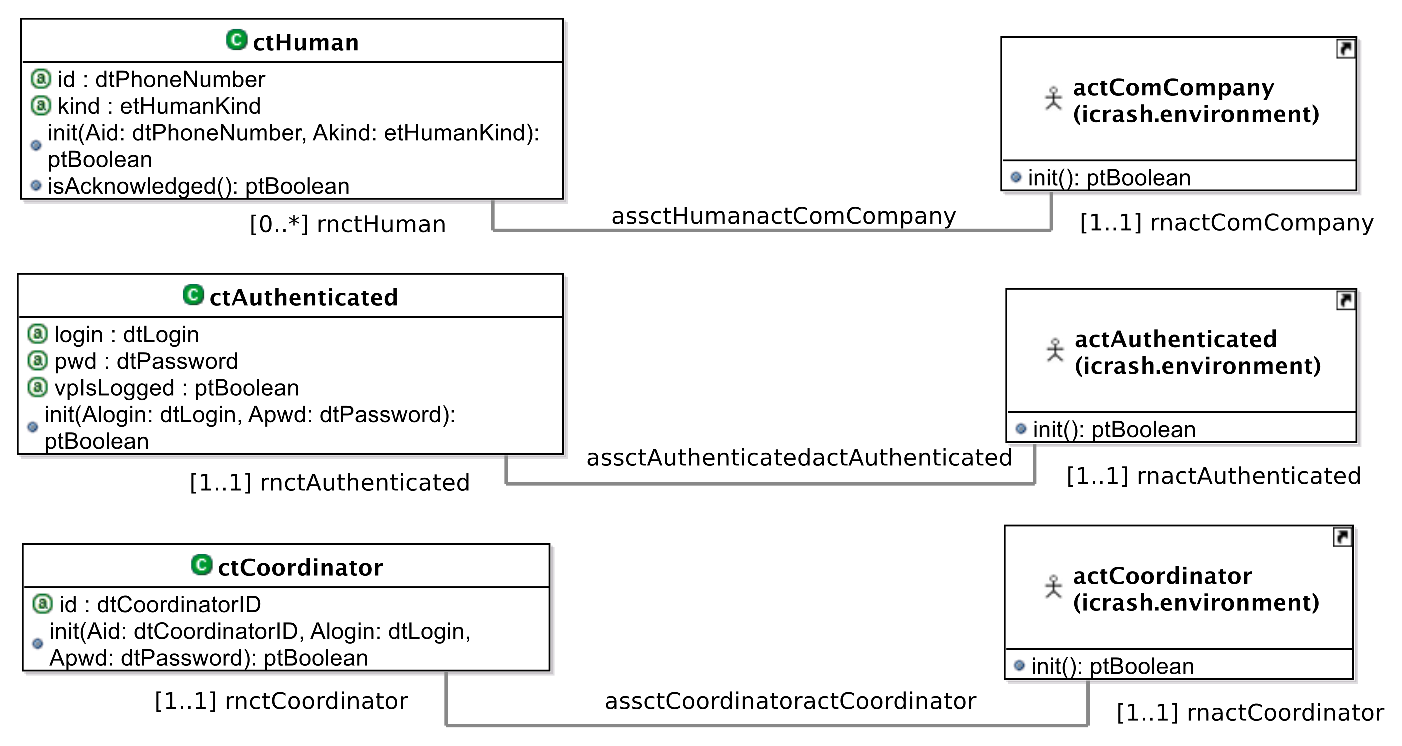
\includegraphics[width=500px]{images/analysis/concept-model/global/PrimaryTypes-Classes/01/cm-pt-ct-gv-01.eps}

% \begin{figure}
% \begin{center}
% \includegraphics[width=\textwidth]{./images/myfigure.eps}
% \end{center}
% \caption{Caption for my figure}
% \label{fig:myfigure}
% \end{figure} 


   

\section{Environment Model}
